%narms.tex, an example driver file for Balkema documents.

%use the following for A4 paper:
\documentclass[12pt,a4paper,twocolumn,fleqn]{narms}

% packages needed
\usepackage{epsfig}
\usepackage{timesmt}

% add here more packages based on the document format
% custom packages
\usepackage{dsfont}
\usepackage{amsmath}
\setlength{\mathindent}{0cm}
\usepackage{subfig}
\usepackage{siunitx}
\usepackage[noabbrev]{cleveref}
\usepackage[font=small,justification=justified,singlelinecheck=false]{caption}



% setting math equation indent from left 0pts

\mathindent=0pt%

% use this for chicaco style reference
% Author references
% IMPORTANT: Author wants to format references in chicaco style Author must use BiBTex
% IMPORTANT: Author wants to format numbered references remove chicaco style file and \bibliographystyle{chicaco}

\usepackage{chicaco}

%  \cite{key}
%    which produces citations with full author list and year.
%    eg. (Brown 1978; Jarke, Turner, Stohl, et al. 1985)

%  \citeNP{key}
%    which produces citations with full author list and year, but without
%    enclosing parentheses:
%    eg. Brown 1978; Jarke, Turner & Stohl 1985

%  \citeA{key}
%    which produces citations with only the full author list.
%    eg. (Brown; Jarke, Turner & Stohl)

%  \citeANP{key}
%    which produces citations with only the full author list, without
%    parentheses eg. Brown; Jarke, Turner & Stohl

%  \citeN{key}
%    which produces citations with the full author list and year, but
%    can be used as nouns in a sentence; no parentheses appear around
%    the author names, but only around the year.
%      eg. Shneiderman (1978) states that......
%    \citeN should only be used for a single citation.

%  \shortcite{key}
%    which produces citations with abbreviated author list and year.

%  \shortciteNP{key}
%    which produces citations with abbreviated author list and year.

%  \shortciteA{key}
%    which produces only the abbreviated author list.

%  \shortciteANP{key}
%    which produces only the abbreviated author list.

%  \shortciteN{key}
%    which produces the abbreviated author list and year, with only the
%    year in parentheses. Use with only one citation.

%  \citeyear{key}
%    which produces the year information only, within parentheses.

%  \citeyearNP{key}
%    which produces the year information only.


%%%%%%%%%%%%%%%%%%%%%%%%%%%%%%%%%%%%%%%%%%%%%%%%%%%%%%%%%%%%%%%%%%%
%%%  All this stuff is from modifying the article.cls for Balkema
%%%  specifications.

%\title{...}
%\author{...}
%use \aff for author affiliations
% use \authornext for from second author
% empty line space between multiple authors
%\abstract{...}
%\maketitle{}

%%%%%%% Style for TABLES
% insert tabular command inside \tabletext{} this will produce tables in 10pts


\begin{document}
\title{Effect of initial volume fraction on the collapse of granular columns in fluid}
\author{{K. Kumar} \\
{\aff{Computational Geomechanics Research Group, Department of Engineering, University of Cambridge, UK}} \\
\\
{\authornext{J-Y. Delenne}}\\
{\aff{IATE, UMR 1208 INRA-CIRAD-Montpellier Supagro-UM2, University of Montpellier 2, France.}} \\
\\
{\authornext{K. Soga}}\\
{\aff{Department of Civil and Environmental Engineering, University of California, Berkeley, USA.}}}

\date{}% No date.

\abstract{This paper investigates the effect of initial volume fraction on the runout characteristics of granular column collapse in a fluid. Two-dimensional sub-grain scale numerical simulations are performed to understand the flow dynamics of granular collapse in a fluid. The Discrete Element (DEM) technique is coupled with the Lattice Boltzmann Method (LBM), for fluid-grain interactions, to understand the evolution of submerged granular flows. The fluid phase is simulated using Multiple-Relaxation-Time LBM (LBM-MRT) for numerical stability. In order to simulate interconnected pore space in 2D, a reduction in the radius of the grains (hydrodynamic radius) is assumed during LBM computations. A parametric analysis is performed to assess the influence of the granular characteristics (initial packing) on the evolution of flow and run-out distances. The volume of the initial packing is changed to simulate different stress conditions while maintaining the same aspect ratio. The influence of the stress condition on the run-out behaviour is studied for different permeabilities. The granular flow dynamics is investigated by analysing the effect of hydroplaning, water entrainment and viscous drag on the granular mass. The mechanism of energy dissipation, the shape of the flow front, water entrainment and evolution of packing density is used to explain the difference in the flow characteristics of loose and dense granular column collapse in a fluid.}

\maketitle

\section{INTRODUCTION}


The flow of dense granular material is a common phenomenon in engineering predictions, such as avalanches, landslides, and debris-flow modelling. Despite the huge amount of research that has gone into describing the behaviour of granular flows, a constitutive equation that describes the overall behaviour of a flowing granular material is still lacking. The initiation and propagation of submarine granular flows depend mainly on the slope, density, and quantity of the material destabilised. Although certain macroscopic models are able to capture the simple mechanical behaviours, the complex physical mechanisms that occur at the grain scale, such as thydrodynamic instabilities, the formation of clusters, collapse, and transport, have largely been ignored~\shortcite{Topin2011}. The momentum transfer between the discrete and the continuous phases significantly affects the dynamics of the flow~\shortcite{Peker2007}. Grain-scale description of the granular material enriches the macro-scale variables,  which poorly account for the local rheology of the materials.  In order to describe the mechanism of saturated and/or immersed granular flows, it is important to consider both the dynamics of the solid phase and the role of the ambient fluid~\shortcite{Denlinger2001}. In particular, when the solid phase reaches a high volume fraction, it is important to consider the strong heterogeneity arising from the contact forces between the grains, the drag interactions which counteract the movement of the grains, and the hydrodynamic forces that reduce the weight of the solids inducing a transition from dense compacted to a dense suspended flow~\shortcite{Meruane2010}. The case of the collapse in presence of an interstitial fluid has been less studied. In this paper, we study the submarine granular flows in the inclined configuration. We study the effect of permeability, density and slope angle on the run-out evolution.
\section{LBM FORMULATION}

The Lattice Boltzmann Method is a `micro-particle' based numerical time-stepping procedure for the solution of incompressible fluid flows. Consider a 2D incompressible fluid flow with density $\rho$ and kinematic viscosity \textit{v}, in a rectangular domain \textit{\textbf{D}}. The fluid domain is divided into a rectangular grid or lattice, with the same spacing \textit{`h'} in both the \textit{x-} and the \textit{y-}directions, as shown in~\cref{fig:D2Q9}. The present study focuses on two-dimensional problems, hence the \textit{D2Q9} momentum discretisation is adopted (see \shortciteN{He1997} for naming convention).

\begin{figure}[htpb]
\centering
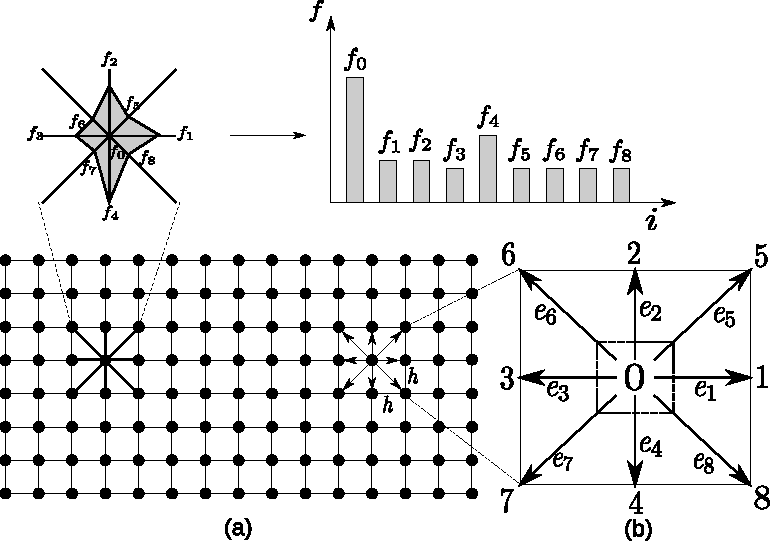
\includegraphics[width=0.45\textwidth]{figs/D2Q9.pdf}
\caption[The Lattice Boltzmann discretisation and D2Q9 scheme]{The Lattice Boltzmann discretisation and D2Q9 scheme: (a) a standard LB lattice and histogram views of the discrete single particle distribution function/direction-specific densities $f_i$; (b) D2Q9 model}
\label{fig:D2Q9}
\end{figure}

The lattice Boltzmann Bhatnagar-Gross-Krook (LGBK) method is capable of simulating various hydrodynamics~\shortcite{Succi2001} and offers intrinsic parallelism. Although LBM is successful in modelling complex fluid systems, such as multiphase flows and suspensions in fluid, the LBM may lead to numerical instability when the dimensionless relaxation time $\tau$ is close to 0.5. The Multi-Relaxation Time Lattice Boltzmann Method (LBM-MRT) overcomes the deficiencies of linearlised single relaxation LBM-BGK, such as fixed Prandtl number (Pr=$\nu/\kappa$), where the thermal conductivity `$\kappa$' is unity~\shortcite{Liu2003a}. The LB-MRT model offers better numerical stability and has more degrees of freedom. In the formulation of the linear Boltzmann equation with multiple relaxation time approximation, the lattice Boltzmann equation is written as:

\begin{align}
&f_{\alpha}(\mathbf{x}+\mathbf{e}_i\Delta_t, t+ \Delta_t)-f_{\alpha}(\mathbf{x},t) \nonumber \\
&\mbox{\qquad\qquad} = -\mathbf{S}_{\alpha i}(f_i(\mathbf{x},t)-f_i^{eq}(\mathbf{x},t)
\end{align}

\noindent where \textbf{S} is collision matrix. The nine eigen values of \textbf{S} are all between 0 and 2 so as to maintain linear stability and the separation of scales, which means that the relaxation times of non-conserved quantities are much faster than the hydrodynamic time scales. The LGBK model is the special case in which the nine relaxation times are all equal and the collision matrix $\mathbf{S}=\frac{1}{\tau}\mathbf{I}$, where \textbf{I} is the identity matrix. The evolutionary progress involves two steps, advection and flux. The advection can be mapped to the momentum space by multiplying through by a transformation matrix \textbf{M} and the flux is still finished in the velocity space. The evolutionary equation of the multi-relaxation time lattice Boltzmann equation is written as:

\begin{align}
&\mathbf{f}(\mathbf{x}+\mathbf{e}_i\Delta_t, t+ \Delta_t)-\mathbf{f}(\mathbf{x},t) \nonumber \\
&\mbox{\qquad\qquad} = -M^{-1}\hat{\mathbf{S}} (\hat{\mathbf{f}}(\mathbf{x},t)-\hat{\mathbf{f}}^{eq}(\mathbf{x},t))
\end{align}

\noindent where \textbf{M} is the transformation matrix mapping a vector \textbf{f} in the discrete velocity space $\mathds{V}=\mathds{R}^b$ to a vector $\hat{\mathbf{f}}$ in the moment space $\mathds{V}=\mathds{R}^b$.

\begin{align}
&\hat{\mathbf{f}} = \mathbf{M}\mathbf{f}\\
&\mathbf{f}(\mathbf{x},t) = \left[f_0(\mathbf{x},t),f_1(\mathbf{x},t),\dots f_8(\mathbf{x},t)\right]^T
\end{align}

The collision matrix $\hat{\mathbf{S}} = MSM^{-1}$ in moment space is a diagonal matrix: $\hat{\mathbf{S}} =\mbox{diag} \left[ s_1, s_2, s_3,\dots s_9  \right]$. The transformation matrix \textbf{M} can be constructed via Gram-Schmidt orthgonalisation procedure. Through the Chapman-Enskog expansion~\shortcite{Du2006}, the incompressible Navier-Stokes equation can be recovered and the viscosity is given as:
\begin{align}
\nu=c_s^2\Delta t(\tau-0.5)
\end{align}
%**************************************************************************

\subsection{Turbulence in Lattice Boltzmann Method}
Modelling fluids with low viscosity like water remains a challenge, necessitating very small values of \textit{h}, and/or $\tau$ very close to 0.5~\shortcite{He1997}. Turbulent flows are characterised by the occurrence of eddies with multiple scales in space, time and energy. In this study, the Large Eddy Simulation (LES) is adopted to solve for turbulent flow problems. The separation of scales is achieved by filtering of the Navier-Stokes equations, from which the resolved scales are directly obtained and unresolved scales are modelled by a one-parameter Smagorinski sub-grid methodology, which assumes that the Reynold's stress tensor is dependent only on the local strain rate~\shortcite{Smagorinsky1963}. The turbulent viscosity $\nu$ is related to the strain rate $S_{ij}$ and a filtered length scale `h' as follows:
\begin{align}
&\mathit{v}_{\mathit{t}}  =  (\mathit{S}_{c}\mathit{h})^{2}\overline{S}; \\
&\overline{S}  = \sqrt{\sum\limits_{\mathit{i,j}}{\tilde{S}_{\mathit{i,j}}\tilde{S}_{\mathit{i,j}}}}
\end{align}
where $\mathit{S}_{c}$ is the Smagorinski constant found to be close to 0.03~\shortcite{yu2005}.

The effect of the unresolved scale motion is taken into account by introducing an effective collision relaxation time scale $\tau_{t}$, so that the total relaxation time $\tau_{*}$ is written as:
\begin{align}
\tau_{*}=\tau + \tau_{t}
\end{align}
where $\tau$ and $\tau_{t}$ are respectively the standard relaxation times corresponding to the true fluid viscosity \textit{v} and the turbulence viscosity $\mathit{v}_{\mathit{t}}$, defined by a sub-grid turbulence model. The new viscosity $\mathit{v}_{*}$ corresponding to $\tau_{*}$ is defined as:
\begin{align}
& \mathit{v}_{*}=\mathit{v}+\mathit{v}_{\mathit{t}}=\frac{1}{3}(\tau+\tau_{t}-\frac{1}{2})\mathit{C}^{2} \Delta \mathit{t}  \\
& \mathit{v}_{\mathit{t}}=\frac{1}{3}\tau_{\mathit{t}}\mathit{C}^{2} \Delta \textit{t}
\end{align}
The Smagorinski model is easy to implement and the Lattice Boltzmann formulation remains unchanged, except for the use of a new turbulence-related viscosity $\tau_{*}$. The component $s_1$ of the collision matrix becomes $s_1 = \frac{1}{\tau+\tau_t}$.
%************************************************************************* %
\section{COUPLED LB - DEM FOR FLUID-PARTICLE INTERACTIONS}
The Lattice Boltzmann approach has the advantage of accommodating large particle sizes and the interaction between the fluid and the moving particles can be modelled through relatively simple fluid - particle interface treatments. Further, employing the Discrete Element Method (DE) to account for the particle/particle interaction naturally leads to a combined LB - DEM solution procedure. The Eulerian nature of the Lattice Boltzmann formulation, together with the common explicit time step scheme of both the Lattice Boltzmann and the Discrete Element makes this coupling strategy an efficient numerical procedure for the simulation of particle-fluid systems~\shortcite{Cook2004}. In order to capture the actual physical behaviour of the fluid-particle system, the boundary condition between the fluid and the particle is modelled as a non-slip boundary condition, i.e. the fluid near the particle should have similar velocity as the particle boundary. The solid particles inside the fluid are represented by lattice nodes. The discrete nature of lattice will result in stepwise representation of the surfaces. Very small lattice spacing is adopted to obtain smoother boundaries.

\section{UNDERWATER GRANULAR FLOWS}
In this study, a 2D poly-disperse system ($d_{max}/d_{min} = 1.8$) of circular discs in fluid was used to understand the behaviour of granular flows on inclined planes (see~\Cref{fig:setup}). The soil column was modelled using 1000 discs of density \SI{2650}{\kg\per\cubic\meter} and a contact friction angle of \SI{26}{\degree}. The collapse of the column was simulated inside a fluid with a density of \SI{1000}{\kg\per\cubic\meter}  and a kinematic viscosity of \SI{1e-6}{\square\meter\per\second}. The choice of a 2D geometry has the advantage of cheaper computational effort than a 3D case, making it feasible to simulate very large systems. A granular column of aspect ratio `a' of 0.8 was used. A hydrodynamic radius r = 0.9R was adopted during the LBM computations. Dry analyses were also performed to study the effect of hydrodynamic forces on the run-out distance.

\begin{figure}[htpb]
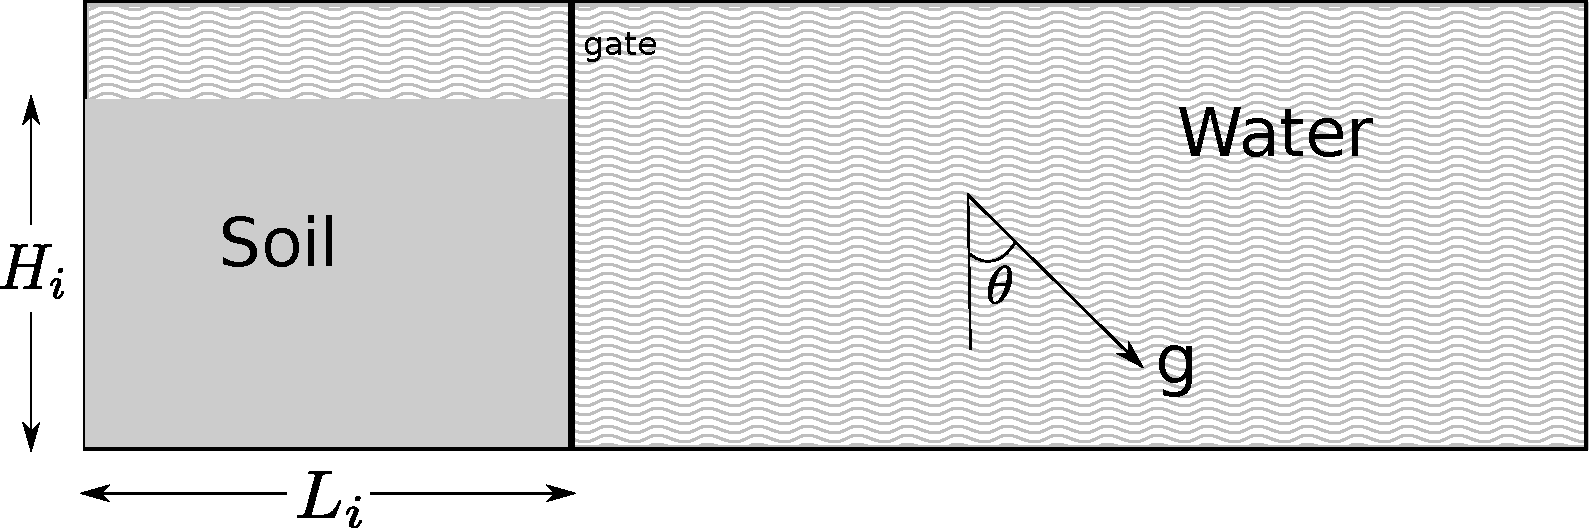
\includegraphics[width=0.97\columnwidth]{figs/geometry.pdf}
\caption{Underwater granular collapse set-up}
\label{fig:setup}
\end{figure}

\subsection{Effect of initial density}

\bibliographystyle{chicaco}
\bibliography{references}

\end{document}
